\section{History}\label{sec:history}
\subsection{First Developments}
In the late 50s of the 19th century \textit{Morton Leonard Heilig}\index{Morton L. Heilig} dreamed about the revolution of cinematic story telling and designed with his \enquote{stereoscopic-television apparatus for individual use}\index{Head-mounted display!Stereoscopic-television apparatus for individual use} the first head-mounted display (see \autoref{fig:Heilig}). The helmet was planned to display stereoscopic images, play surround sound and even add smell to the sensory experience, but was never actual built. His ideas were ahead of their time and could not yet be realized with the technology of the time (compare with \cite[p.3]{Toennis.2010} and \cite[p.4 et seq.]{Burdea.2003}). 

In the decades to follow, several attempts to bring input and display devices for virtual reality onto the consumer market failed due to their high costs and their lack of software. In 1992, \textit{Jaron Lanier}\index{Jaron Lanier} and his company \textit{VPL Research} released the \textit{DataGlove}\footnote{The \textit{datagloves}\index{Dataglove} (also called \textit{wire-} or \textit{cybergloves}) are another step into more immersive input devices, since hand gestures can be directly used to interact with the virtual world.}\index{Dataglove!DataGlove} at the unaffordable prize point of \$9000 USD. The low number of games for \textit{Nintendo's} cheaper \textit{PowerGlove}\index{Dataglove!PowerGlove} led to its discontinuation in 1993 soon after its introduction (\cite[p.8 et seq.]{Burdea.2003} and \cite[p.19 et seq.]{Doerner.2013}).

\begin{figure}[htbp]
		\centering
		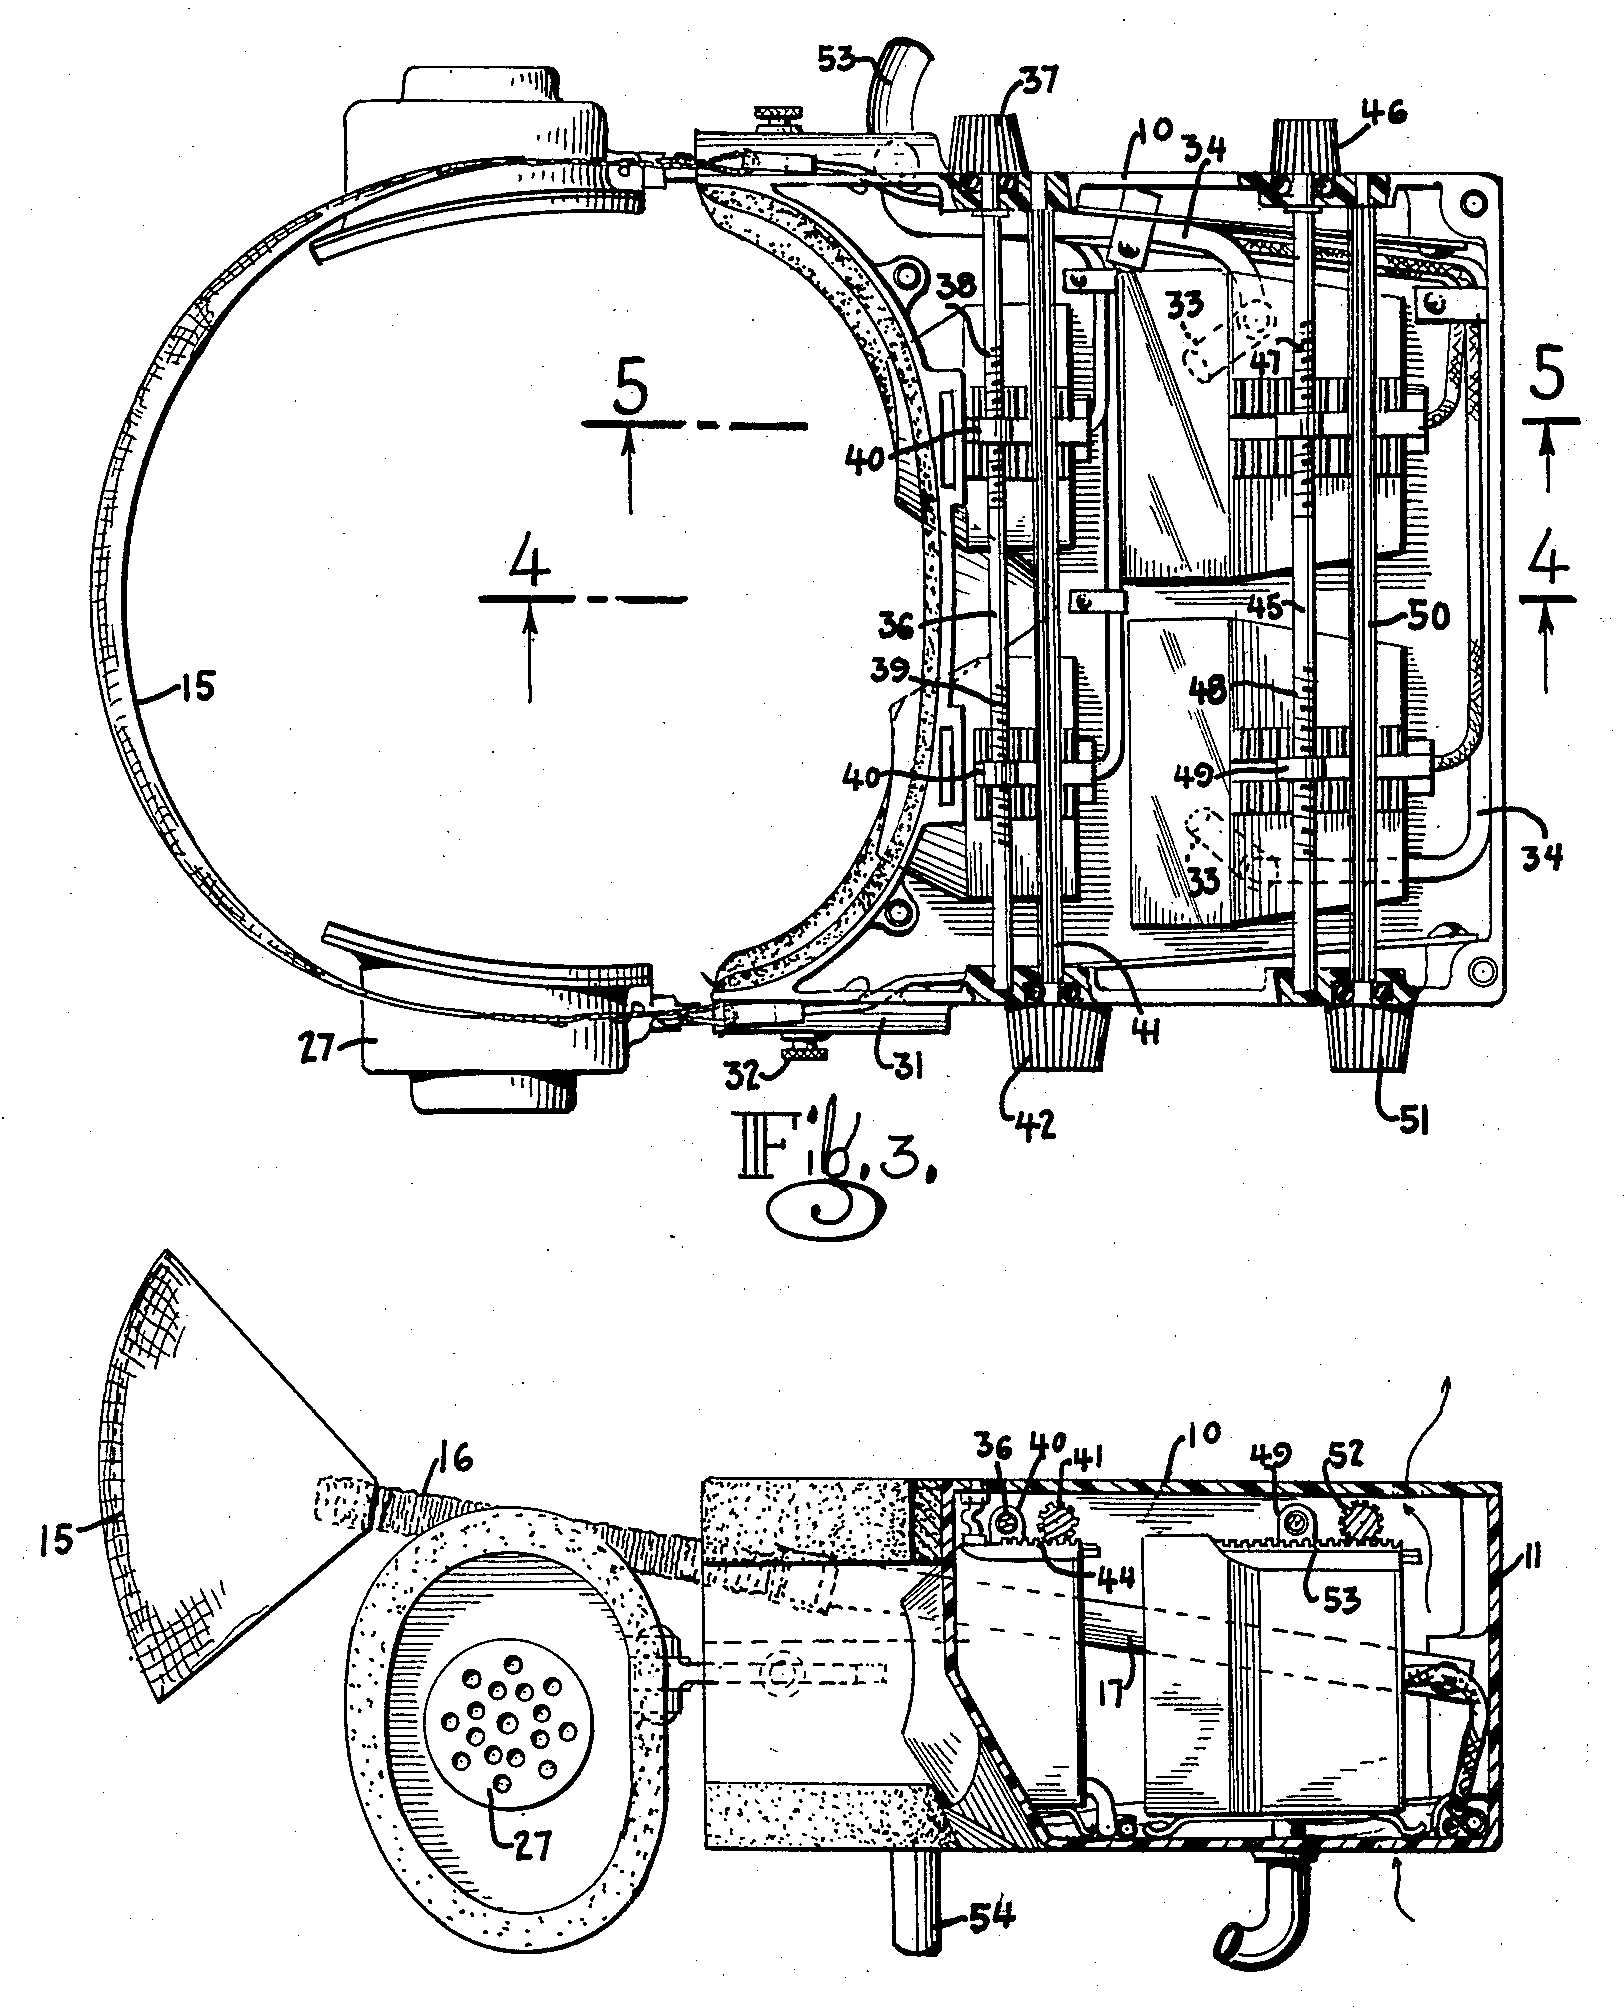
\includegraphics[width=0.4\textwidth]{figures/Heilig_HMD}
		\caption[Stereoscopic-television apparatus for individual use]{Morton Heilig's stereoscopic-television apparatus for individual use (\textit{source: \cite{Heilig.1957}}).}
		\label{fig:Heilig}
\end{figure}

\subsection{Disappointments}
The 80s and 90s were characterized by heavily marketed products, that ultimately disappointed the users and failed to live up to the \enquote{mediahype}. The expectations for virtual reality applications were too high and the technological development was not fast enough. The hardware was too costly\footnote{The fastest graphics system, the \textit{Reality Engine} by \textit{Silicon Graphics}, cost \$100,000 USD at its release in the 1990s(\cite[p.10]{Burdea.2003}).}, the market for VR was too small and there were no investment funds available for companies. These deficits led to the bankruptcy of many companies and caused a serious crisis for the VR industry (\cite[p.10]{Burdea.2003}). 

With the improvement of computer hardware in the late 90s, the speed of graphics computation began to meet the requirements for VR and the hardware was finally affordable for consumers (\cite[p.10 et seq.]{Burdea.2003}, \cite{Doerner.2013} and \cite[p.3]{Toennis.2010}).

\subsection{Today's Usage of Computer Vision}\label{ssec:Today}
Fortunately, due to recent successes in the industry the computer vision plays an increasingly important role in many fields. \textit{David Lowe}, Senior Research Scientist at Google Seattle, separated today's most relevant industrial applications for computer vision into the following categories\footnote{Although he states that his list is not complete and not up-to-date, it can be used as an overview. Go to his homepage to read more about specific applications: \cite{Lowe.2016}} (freely adapted from \cite{Lowe.2016}): 

\begin{description}
\item [Automotive driver assistance and traffic management,]\hfill \\ such as visual warning systems and real-time traffic management.
\item [Eye and head tracking,]\hfill \\ which is also included in head-mounted displays.
\item [Film and video,]\hfill \\ e.g. tracking of the ball in sports for sport analysis or motion tracking systems for animated movies.
\item [Gesture recognition,]\hfill \\ such as full-body motion sensing with the Mircosoft Kinect and the use of gesture recognition as computer inputs for gaming or other computer-related activities.
\item [Industrial automation and inspection,]\hfill \\ like systems for inspection and process control in the electronic or food and agriculture industry. 
\item [Medical and biomedical,]\hfill \\ e.g. the detection and tracking of markers in real-time stereo vision for surgeons.
\item [Object recognition and AR for mobile devices,]\hfill \\ including real-time product recognition and image refinement applications, such as face-swapping apps.
\item [Photography,]\hfill \\ e.g. automated panorama stitching for multiple images.
\item [Safety monitoring,]\hfill \\ monitoring of areas to warn of accidents, e.g. in swimming pools.
\item [Security and biometrics,]\hfill \\ detection and counting of people for security purposes, fingerprint or license plate recognition.
\item [3-D modeling,]\hfill \\ 3-D scanning of objects or the 3-D reconstruction from a number of photographs. 
\item [Web and cloud applications,]\hfill \\ such as image retrieval based on content. 
\end{description}

Regarding all these examples, the entertainment industry seems to be the slowest candidate, which is partly owed to its users high expectations regarding the (graphics) quality. 
